\chapter{Statistiques descriptives}

\section{Vocabulaire et présentation d'une série}

\begin{defin}[Vocabulaire de base]
	\textbf{Population et individu :} L'ensemble étudié en statistiques est appelé la \textbf{population}. Chaque élément qui constitue cet ensemble est un \textbf{individu}.

	\textbf{Caractère :} C'est la propriété ou la grandeur étudiée sur chaque individu.
	\begin{itemize}
		\item Un caractère est dit \textbf{qualitatif} lorsque ses valeurs (appelées modalités) ne sont pas des nombres (ex. : couleur des yeux, filière).
		\item Un caractère est dit \textbf{quantitatif} lorsqu'il prend des valeurs numériques.
		      \begin{itemize}
			      \item Il est \textbf{discret} si les valeurs sont \og{}isolées\fg{} (ex. : nombre d'enfants)
			      \item Il est \textbf{continu} si les valeurs sont regroupées en intervalles appelés \textbf{classes} (ex. : taille en $\text{cm}$)
		      \end{itemize}
	\end{itemize}
\end{defin}

\begin{defin}[Effectifs, fréquences et cumul]
	Soit une série statistique de $k$ valeurs distinctes $x_1, x_2, \dots, x_k$ (ordonnées dans l'ordre croissant).
	\begin{itemize}
		\item L'\textbf{effectif} $n_i$ associé à la valeur $x_i$ est le nombre d'individus possédant cette valeur.
		\item L'\textbf{effectif total} est la somme de tous les effectifs :
		      \[
			      N = n_1 + n_2 + \dots + n_k \qquad = \displaystyle\sum_{i=1}^k n_i
		      \]
		\item La \textbf{fréquence} $f_i$ associée à la valeur $x_i$ est le quotient $f_i = \dfrac{n_i}{N}$. La somme des fréquences est égale à $1$ (ou $100\,\%$).
		\item L'\textbf{effectif cumulé croissant (E.C.C.)} associé à la valeur $x_i$ est la somme des effectifs de toutes les valeurs inférieures ou égales à $x_i$.
		\item La \textbf{fréquence cumulée croissante (F.C.C.)} associée à la valeur $x_i$ est la somme des fréquences de toutes les valeurs inférieures ou égales à $x_i$.
	\end{itemize}
\end{defin}

\begin{ex}[Présentation des données sous forme de tableau]
	Voici une série de notes obtenues par un groupe d'élèves :

	\[
		4 \ ; \ 6 \ ; \ 7 \ ; \ 12 \ ; \ 12 \ ; \ 17 \ ; \ 18 \ ; \ 18
	\]

	L'effectif total est $N = 8$.

	\begin{center}
		\rnc{\arraystretch}{1.5}
		\begin{tabular}{|r|c|c|c|c|c|c|}
			\hline
			\rowcolor{gray!30}Notes $x_i$          & 4              & 6              & 7              & 12             & 17             & 18             \\ \hline
			Effectifs $n_i$                        & 1              & 1              & 1              & 2              & 1              & 2              \\ \hline
			E.C.C.                                 & 1              & 2              & 3              & 5              & 6              & 8              \\ \hline
			\rule[-4mm]{0mm}{11mm}Fréquences $f_i$ & $\dfrac{1}{8}$ & $\dfrac{1}{8}$ & $\dfrac{1}{8}$ & $\dfrac{2}{8}$ & $\dfrac{1}{8}$ & $\dfrac{2}{8}$ \\ \hline
			\rule[-4mm]{0mm}{11mm}F.C.C.           & $\dfrac{1}{8}$ & $\dfrac{2}{8}$ & $\dfrac{3}{8}$ & $\dfrac{5}{8}$ & $\dfrac{6}{8}$ & $\dfrac{8}{8}$ \\ \hline
		\end{tabular}
	\end{center}
\end{ex}

\section{Caractéristiques de position}

Les caractéristiques de position (ou de tendance centrale) résument une série statistique par une valeur numérique représentative.

\subsection{Moyenne}

\begin{defin}[Moyenne pondérée]
	La \textbf{moyenne} d'une série statistique de valeurs $x_1, x_2, \dots, x_k$ affectées des effectifs $n_1, n_2, \dots, n_k$ est notée $\bar{x}$. Elle est définie par :

	\[
		\bar{x} = \dfrac{n_1 x_1 + n_2 x_2 + \dots + n_k x_k}{N} \qquad = \dfrac{1}{N} \sum_{i=1}^k n_i x_i
	\]

	Dans le cas d'un caractère continu regroupé en classes $[a ; b[$, on effectue le calcul en remplaçant chaque classe par son centre $\dfrac{a+b}{2}$.
\end{defin}

\begin{ex}[Calcul d'une moyenne simple et pondérée]
	On étudie le nombre de frères et sœurs des $21$ élèves d'une classe de 1STMG :
	\[
		0 \ ; \ 0 \ ; \ 0 \ ; \ 0 \ ; \ 0 \ ; \ 1 \ ; \ 1 \ ; \ 1 \ ; \ 1 \ ; \ 1 \ ; \ 1 \ ; \ 1 \ ; \ 1 \ ; \ 2 \ ; \ 2 \ ; \ 2 \ ; \ 2 \ ; \ 3 \ ; \ 3 \ ; \ 3 \ ; \ 4
	\]

	\begin{enumerate}
		\item \textbf{Calcul non pondéré (moyenne simple) :}

		      On additionne directement l'ensemble des $21$ valeurs individuelles :
		      \[
			      \bar{x} = \dfrac{0 + 0 + 0 + 0 + 0 + 1 + 1 + 1 + 1 + 1 + 1 + 1 + 1 + 2 + 2 + 2 + 2 + 3 + 3 + 3 + 4}{21} = \dfrac{29}{21} \approx 1{,}38
		      \]

		\item \textbf{Calcul pondéré (à partir du tableau d'effectifs) :}

		      En regroupant les valeurs identiques avec leur effectif $n_i$ associé :
		      \begin{center}
			      \rnc{\arraystretch}{1.3}
			      \begin{tabular}{|r|c|c|c|c|c|} \hline
				      \rowcolor{gray!30} Nombre de frères et sœurs $x_i$ & 0 & 1 & 2 & 3 & 4 \\ \hline
				      Effectifs $n_i$                                    & 5 & 8 & 4 & 3 & 1 \\ \hline
			      \end{tabular}
		      \end{center}

		      Le calcul devient :
		      \[
			      \bar{x} = \dfrac{5 \times 0 + 8 \times 1 + 4 \times 2 + 3 \times 3 + 1 \times 4}{21} = \dfrac{29}{21} \approx 1{,}38
		      \]
	\end{enumerate}

	On vérifie bien que les deux méthodes mènent au même résultat.
\end{ex}

\begin{ex}[Calcul de la moyenne d'un caractère continu]
	Dans une classe de 1STMG, on mesure la taille des élèves (en $\text{cm}$) regroupée par classes d'amplitude $5\text{ cm}$ :

	\begin{center}
		\rnc{\arraystretch}{1.3}
		\begin{tabular}{|c|c|c|c|}\hline
			\rowcolor{gray!30}
			Taille $I_i$ (en $\text{cm}$) & Centre $c_i$ & Effectif $n_i$ & $n_i \times c_i$              \\ \hline
			$[160 ; 165[$                 & $162{,}5$    & 4              & $4 \times 162{,}5 = 650$      \\ \hline
			$[165 ; 170[$                 & $167{,}5$    & 9              & $9 \times 167{,}5 = 1507{,}5$ \\ \hline
			$[170 ; 175[$                 & $172{,}5$    & 8              & $8 \times 172{,}5 = 1380$     \\ \hline
			$[175 ; 180[$                 & $177{,}5$    & 3              & $3 \times 177{,}5 = 532{,}5$  \\ \hline
			\textbf{Total}                & -            & $N = 24$       & $4070$                        \\ \hline
		\end{tabular}
	\end{center}

	On calcule la taille moyenne estimée en appliquant la formule de la moyenne pondérée aux centres des classes :
	\[
		\bar{x} = \dfrac{4 \times 162{,}5 + 9 \times 167{,}5 + 8 \times 172{,}5 + 3 \times 177{,}5}{24} = \dfrac{4070}{24} \approx 169{,}58\text{ cm}
	\]
\end{ex}

\newpage

\begin{prop}[Linéarité de la moyenne]
	Soit une série de moyenne $\bar{x}$ et deux réels $a$ et $b$.
	\begin{itemize}
		\item Si on multiplie toutes les valeurs de la série par $a$, la nouvelle moyenne devient $a\bar{x}$.
		\item Si on ajoute $b$ à toutes les valeurs de la série, la nouvelle moyenne devient $\bar{x} + b$.
		\item De façon générale, les valeurs $a x_i + b$ ont pour moyenne $a\bar{x} + b$.
	\end{itemize}
\end{prop}

\begin{methode}[Utiliser la linéarité de la moyenne]
	Un relevé du prix au litre d'essence dans 5 stations donne :
	\[
		1{,}50\text{ \euro}, 1{,}44\text{ \euro}, 1{,}51\text{ \euro}, 1{,}62\text{ \euro} \text{ et } 1{,}58\text{ \euro}
	\]

	\begin{enumerate}
		\item Calculer le prix moyen initial.
		\item Calculer le prix moyen après une augmentation générale de $30\,\%$.
		\item Calculer le prix moyen final après une remise de $0{,}15\text{ \euro}$ par litre.
	\end{enumerate}

	\begin{correction}
		\nline
		\begin{enumerate}
			\item Prix moyen initial : $\bar{x} = \dfrac{1{,}50 + 1{,}44 + 1{,}51 + 1{,}62 + 1{,}58}{5} = \dfrac{7{,}65}{5} = 1{,}53\text{ \euro}$.
			\item Augmenter de $30\,\%$ revient à multiplier par $1{,}30$. Par linéarité :
			      \[
				      \bar{x}_{\text{hausse}} = 1{,}53 \times 1{,}30 = 1{,}989\text{ \euro}
			      \]

			\item Soustraire $0{,}15\text{ \euro}$ à chaque valeur revient à soustraire $0{,}15$ à la moyenne :
			      \[
				      \bar{x}_{\text{final}} = 1{,}989 - 0{,}15 = 1{,}839\text{ \euro}
			      \]
		\end{enumerate}
	\end{correction}
\end{methode}

\subsection{Médiane}

\begin{defin}[Médiane]
	La \textbf{médiane} d'une série ordonnée dans l'ordre croissant, notée $M_e$, est une valeur qui partage la série en deux groupes de même effectif :
	\begin{itemize}
		\item Au moins $50\,\%$ des valeurs sont inférieures ou égales à $M_e$, ...
		\item ... et au moins $50\,\%$ des valeurs sont supérieures ou égales à $M_e$.
	\end{itemize}
\end{defin}

\begin{methode}[Déterminer la médiane d'une série discrète]
	Soit $N$ l'effectif total de la série rangée dans l'ordre croissant.
	\begin{itemize}
		\item \textbf{Si $N$ est impair ($N = 2p + 1$) :} la médiane est la valeur de rang $p + 1$.
		\item \textbf{Si $N$ est pair ($N = 2p$) :} la médiane est la moyenne arithmétique entre la valeur de rang $p$ et la valeur de rang $p + 1$.
	\end{itemize}

	\begin{correction}
		\nline
		\begin{itemize}
			\item \textbf{Série A ($N = 9$) :} $9 \ ; \ 10 \ ; \ 10 \ ; \ 11 \ ; \ \boxed{~\mathbf{12}~} \ ; \ 12 \ ; \ 13 \ ; \ 14 \ ; \ 15$.

			      $N$ est impair ($9 = 2 \times 4 + 1$). La médiane est la $5^{\text{e}}$ valeur : $M_e = 12$.
			\item \textbf{Série B ($N = 8$) :} $4 \ ; \ 6 \ ; \ 8 \ ; \ \boxed{~\mathbf{11}~} \ ; \ \boxed{~\mathbf{12}~} \ ; \ 17 \ ; \ 18 \ ; \ 18$.

			      $N$ est pair ($8 = 2 \times 4$). La médiane est la moyenne entre la $4^{\text{e}}$ et la $5^{\text{e}}$ valeur :
			      \[
				      M_e = \dfrac{11 + 12}{2} = 11{,}5
			      \]
		\end{itemize}
	\end{correction}
\end{methode}

\newpage

\begin{ex}[Déterminer la médiane à l'aide des effectifs cumulés croissants]
	On relève la pointure des $20$ joueurs d'un club de basket :

	\begin{center}
		\rnc{\arraystretch}{1.3}
		\begin{tabular}{|r|c|c|c|c|c|c|c|c|c|} \hline
			\rowcolor{gray!30} Pointure $x_i$ & 39 & 40 & 41 & 42 & 43 & 44 & 45 & 46 & 47 \\ \hline
			Effectifs $n_i$                   & 1  & 2  & 3  & 4  & 5  & 2  & 1  & 1  & 1  \\ \hline
			E.C.C.                            & 1  & 3  & 6  & 10 & 15 & 17 & 18 & 19 & 20 \\ \hline
		\end{tabular}
	\end{center}

	\textbf{Méthode :}
	\begin{itemize}
		\item L'effectif total est $N = 20$, ce qui est un nombre pair ($20 = 2 \times 10$).
		\item La médiane est la moyenne entre la $10^{\text{e}}$ et la $11^{\text{e}}$ valeur.
		\item On lit dans la ligne des \textbf{E.C.C.} :
		      \begin{itemize}
			      \item La $10^{\text{e}}$ valeur est la dernière de la tranche des pointures 42 (E.C.C. = 10).

			            Donc la $10^{\text{e}}$ valeur vaut $42$.
			      \item La $11^{\text{e}}$ valeur entre dans la tranche suivante, celle des pointures 43 (E.C.C. passe de 10 à 15).

			            Donc la $11^{\text{e}}$ valeur vaut $43$.
		      \end{itemize}
	\end{itemize}

	On calcule la médiane :
	\[
		M_e = \dfrac{42 + 43}{2} = 42{,}5
	\]

	Au moins $50\,\%$ des joueurs ont une pointure inférieure ou égale à $42{,}5$.
\end{ex}

\section{Caractéristiques de dispersion}

Les caractéristiques de dispersion mesurent l'étalement des valeurs autour d'une valeur centrale.

\subsection{Étendue, quartiles et écart interquartile}

\begin{defin}[Étendue]
	L'\textbf{étendue} d'une série statistique est la différence entre la plus grande valeur et la plus petite valeur observée :
	\[
		\text{Étendue} = x_{\max} - x_{\min}
	\]
\end{defin}

\begin{ex}[Calcul de l'étendue]
	On reprend le tableau de la série des pointures des $20$ joueurs de basket :

	\begin{center}
		\rnc{\arraystretch}{1.3}
		\begin{tabular}{|r|c|c|c|c|c|c|c|c|c|} \hline
			\rowcolor{gray!30} Pointure $x_i$ & 39 & 40 & 41 & 42 & 43 & 44 & 45 & 46 & 47 \\ \hline
			Effectifs $n_i$                   & 1  & 2  & 3  & 4  & 5  & 2  & 1  & 1  & 1  \\ \hline
		\end{tabular}
	\end{center}

	La plus grande pointure est $x_{\max} = 47$ et la plus petite est $x_{\min} = 39$.
	\[
		\text{Étendue} = 47 - 39 = 8
	\]

	L'écart maximal de pointure entre deux joueurs de cette équipe est de $8$ pointures.
\end{ex}

\begin{defin}[Quartiles]
	Soit une série statistique ordonnée dans l'ordre croissant et d'effectif total $N$.
	\begin{itemize}
		\item Le \textbf{premier quartile}, noté $Q_1$, est la plus petite valeur de la série telle qu'au moins $25\,\%$ (un quart) des valeurs lui soient inférieures ou égales.
		\item Le \textbf{troisième quartile}, noté $Q_3$, est la plus petite valeur de la série telle qu'au moins $75\,\%$ (trois quarts) des valeurs lui soient inférieures ou égales.
		\item L'\textbf{écart interquartile} est le nombre $Q_3 - Q_1$. Il mesure la dispersion de $50\,\%$ des valeurs centrales.
	\end{itemize}
\end{defin}

\begin{methode}[Calculer les quartiles]
	Pour déterminer $Q_1$ et $Q_3$ :
	\begin{enumerate}[itemsep=2mm]
		\item On calcule $\dfrac{N}{4}$. Si ce nombre n'est pas un entier, on l'arrondit à l'entier supérieur $k$.

		      $Q_1$ est la $k^{\text{e}}$ valeur de la série ordonnée.
		\item On calcule $\dfrac{3N}{4}$. Si ce nombre n'est pas un entier, on l'arrondit à l'entier supérieur $p$.

		      $Q_3$ est la $p^{\text{e}}$ valeur de la série ordonnée.
	\end{enumerate}

	\begin{correction}
		Soit la série ordonnée de $N = 9$ notes : $9 \ ; \ 10 \ ; \ 10 \ ; \ 11 \ ; \ 12 \ ; \ 12 \ ; \ 13 \ ; \ 14 \ ; \ 15$.

		\begin{itemize}[itemsep=2mm]
			\item $\dfrac{1}{4}\times 9 = 2{,}25 \implies$ le premier entier supérieur est $3$. $Q_1$ est la $3^{\text{e}}$ valeur, soit $Q_1 = 10$.
			\item $\dfrac{3}{4}\times 9 = 6{,}75 \implies$ le premier entier supérieur est $7$. $Q_3$ est la $7^{\text{e}}$ valeur, soit $Q_3 = 13$.
			\item L'écart interquartile vaut $Q_3 - Q_1 = 13 - 10 = 3$.
		\end{itemize}
	\end{correction}
\end{methode}

\subsection{Diagramme en boîte (ou boîte à moustaches)}

\begin{defin}[Diagramme en boîte]
	Le \textbf{diagramme en boîte} (ou \textbf{boîte à moustaches}) est une représentation graphique de la dispersion d'une série statistique.

	Il s'appuie sur $5$ valeurs caractéristiques :
	\begin{itemize}
		\item Les valeurs extrêmes : le minimum $x_{\min}$ et le maximum $x_{\max}$ ;
		\item Les caractéristiques de position : le premier quartile $Q_1$, la médiane $M_e$ et le troisième quartile $Q_3$.
	\end{itemize}
\end{defin}

\begin{rem}
	\nline
	\begin{itemize}
		\item La \og{}boîte\fg{} centrale (rectangle) est délimitée par $Q_1$ et $Q_3$.

		      Sa largeur correspond à l'\textbf{écart interquartile} ($Q_3 - Q_1$), qui contient $50\,\%$ des valeurs centrales de la population.
		\item Le trait vertical à l'intérieur de la boîte indique la position de la \textbf{médiane} $M_e$.
		\item Les \og{}moustaches\fg{} (segments aux extrémités) s'étendent du minimum $x_{\min}$ jusqu'à $Q_1$, et de $Q_3$ jusqu'au maximum $x_{\max}$.
	\end{itemize}
\end{rem}

\begin{ex}[Tracer un diagramme en boîte]
	On reprend la série des pointures des $20$ joueurs de basket ($x_{\min} = 39$, $Q_1 = 41$, $M_e = 42{,}5$, $Q_3 = 43$, $x_{\max} = 47$) :

	\begin{center}
		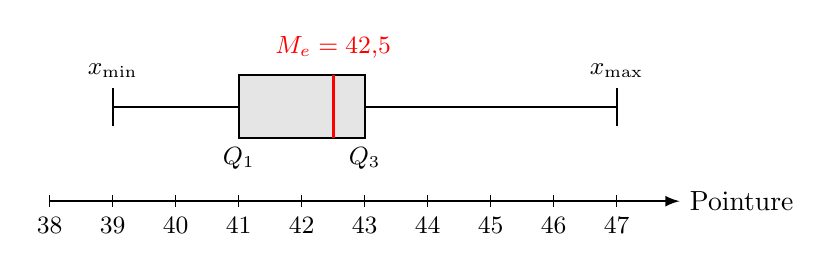
\begin{tikzpicture}[scale=0.8]
			\draw[->, >=latex, thick] (38,0) -- (48,0) node[right] {Pointure};
			\foreach \x in {38,39,...,47} { \draw (\x,0.1) -- (\x,-0.1) node[below] {\small \x}; }
			\draw[thick, fill=gray!20] (41,1) rectangle (43,2);
			\draw[very thick, red] (42.5,1) -- (42.5,2) node[above=2pt, red] {\small $M_e = 42{,}5$};
			\draw[thick] (39,1.5) -- (41,1.5);
			\draw[thick] (43,1.5) -- (47,1.5);
			\draw[thick] (39,1.2) -- (39,1.8) node[above] {\small $x_{\min}$};
			\draw[thick] (47,1.2) -- (47,1.8) node[above] {\small $x_{\max}$};
			\node[below] at (41,1) {\small $Q_1$};
			\node[below] at (43,1) {\small $Q_3$};
		\end{tikzpicture}
	\end{center}

	\textbf{Interprétation :}
	\begin{itemize}
		\item La boîte centrale contient $50\,\%$ des effectifs : au moins la moitié des joueurs chaussent une pointure comprise entre $41$ ($Q_1$) et $43$ ($Q_3$).
		\item Au moins $50\,\%$ des joueurs ont une pointure inférieure ou égale à $42{,}5$ ($M_e$).
	\end{itemize}
\end{ex}

\newpage

\subsection{Variance et écart-type}

\begin{defin}[Variance et écart-type]
	Soit une série statistique de moyenne $\bar{x}$, dont les valeurs $x_i$ ont pour effectifs $n_i$ (avec un effectif total $N$).
	\begin{itemize}
		\item La \textbf{variance}, notée $V$, est la moyenne des carrés des écarts à la moyenne :
		      \[
			      V = \dfrac{n_1\pa{x_1 - \bar{x}}^2 + n_2\pa{x_2 - \bar{x}}^2 + \dots + n_k\pa{x_k - \bar{x}}^2}{N}
		      \]
		\item L'\textbf{écart-type}, noté $\sigma$, est la racine carrée de la variance :
		      \[
			      \sigma = \sqrt{V}
		      \]
	\end{itemize}
\end{defin}

\begin{remarque}
	L'écart-type s'exprime dans la même unité que les données de la série, contrairement à la variance.

	Il mesure la dispersion des valeurs autour de la moyenne arithmétique : plus $\sigma$ est petit, plus la série est \textbf{concentrée} autour de sa \textbf{moyenne}.
\end{remarque}

\begin{methode}[Calculer la variance et l'écart-type]
	On considère la distribution suivante :
	\begin{center}
		\rnc{\arraystretch}{1.2}
		\begin{tabular}{|c|c|c|c|c|} \hline
			\cellcolor{gray!30} $x_i$ & 1 & 2 & 3 & 4 \\ \hline
			\cellcolor{gray!30} $n_i$ & 5 & 9 & 3 & 1 \\ \hline
		\end{tabular}
	\end{center}

	\begin{correction}
		\nline
		\begin{enumerate}
			\item \textbf{Calcul de la moyenne $\bar{x}$ :}

			      \[
				      N = 5 + 9 + 3 + 1 = 18 \quad \text{et} \quad \bar{x} = \dfrac{5 \times 1 + 9 \times 2 + 3 \times 3 + 1 \times 4}{18} = \dfrac{36}{18} = 2
			      \]

			\item \textbf{Calcul de la variance $V$ via le tableau d'écarts :}
			      \ms
			      \begin{center}
				      \rnc{\arraystretch}{1.2}
				      \begin{tabular}{|c|c|c|c|c|} \hline
					      \cellcolor{gray!30} Valeur $x_i$           & 1                & 2                & 3                & 4                \\ \hline
					      \cellcolor{gray!30} Effectif $n_i$         & 5                & 9                & 3                & 1                \\ \hline
					      \cellcolor{gray!30} $x_i - \bar{x}$        & $-1$             & $0$              & $1$              & $2$              \\ \hline
					      \cellcolor{gray!30} $(x_i - \bar{x})^2$    & $1$              & $0$              & $1$              & $4$              \\ \hline
					      \cellcolor{gray!30} $n_i(x_i - \bar{x})^2$ & $5 \times 1 = 5$ & $9 \times 0 = 0$ & $3 \times 1 = 3$ & $1 \times 4 = 4$ \\ \hline
				      \end{tabular}
			      \end{center}

			      \ms

			      On effectue le calcul de la variance grâce à la dernière ligne :
			      \[
				      V = \dfrac{5 + 0 + 3 + 4}{18} = \dfrac{12}{18} = \dfrac{2}{3} \approx 0{,}67
			      \]

			\item \textbf{Calcul de l'écart-type $\sigma$ :}
			      \[
				      \sigma = \sqrt{\dfrac{2}{3}} \approx 0{,}82
			      \]
		\end{enumerate}
	\end{correction}
\end{methode}

\newpage

\section{Représentations graphiques}

Le choix de la représentation graphique dépend de la nature du caractère étudié (discret ou continu) et de ce que l'on cherche à mettre en évidence.

\subsection{Caractère discret : Diagramme en bâtons et diagramme circulaire}

\begin{defin}[Diagramme en bâtons]
	Pour une série statistique à \textbf{caractère discret}, on représente chaque valeur par un bâton vertical dont la hauteur est proportionnelle à l'effectif (ou à la fréquence).
\end{defin}

\begin{ex}[Diagramme en bâtons]
	On reprend le nombre de frères et sœurs des $21$ élèves de Première STMG :

	\begin{center}
		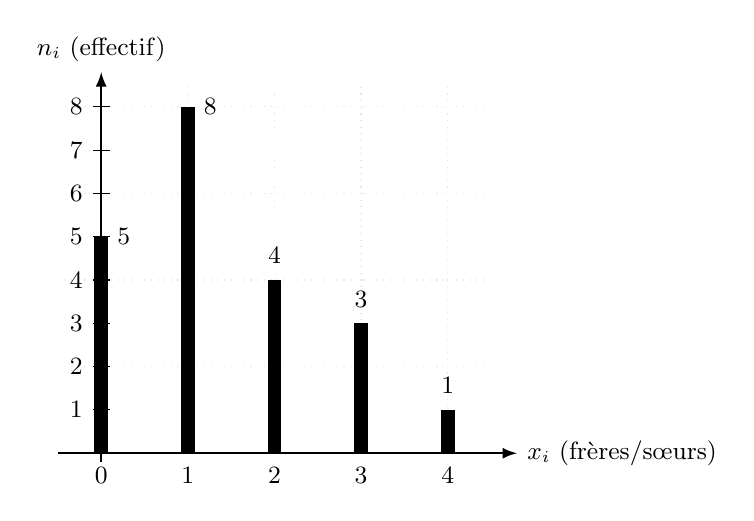
\begin{tikzpicture}[scale=1.1, baseline=(current bounding box.center), y=5mm]
			\draw[gray!20, dotted] (-0.5,0) grid (4.5,8.5);
			\draw[->, >=latex, thick] (-0.5,0) -- (4.8,0) node[right] {\small $x_i$ (frères/sœurs)};
			\draw[->, >=latex, thick] (0,-0.2) -- (0,8.8) node[above] {\small $n_i$ (effectif)};
			\foreach \y in {1,2,...,8} { \draw (0.1,\y) -- (-0.1,\y) node[left] {\small \y}; }
			\draw[line width=5pt] (0,0) -- (0,5) node[above,right] {\small 5};
			\draw[line width=5pt] (1,0) -- (1,8) node[above,right] {\small 8};
			\draw[line width=5pt] (2,0) -- (2,4) node[above] {\small 4};
			\draw[line width=5pt] (3,0) -- (3,3) node[above] {\small 3};
			\draw[line width=5pt] (4,0) -- (4,1) node[above] {\small 1};
			\foreach \x in {0,1,2,3,4} { \node[below] at (\x,-0.1) {\small \x}; }
		\end{tikzpicture}
	\end{center}
\end{ex}

\begin{defin}[Diagramme circulaire (ou « camembert »)]
	Un \textbf{diagramme circulaire} partage un disque en secteurs dont la mesure de l'angle (en degrés) est proportionnelle à l'effectif ou à la fréquence de chaque modalité :
	\[
		\text{Angle (en degrees)} = \text{Fréquence} \times 360^\circ = \dfrac{n_i}{N} \times 360^\circ
	\]
\end{defin}

\begin{ex}[Diagramme circulaire]
	Pour une répartition de $24$ élèves selon leur filière de spécialité :
	\begin{itemize}
		\item Mercatique : $12$ élèves ($50\,\% \rightarrow 180^\circ$)
		\item Gestion-Finance : $8$ élèves ($\approx 33{,}3\,\% \rightarrow 120^\circ$)
		\item R.H. : $4$ élèves ($\approx 16{,}7\,\% \rightarrow 60^\circ$)
	\end{itemize}

	\begin{center}
		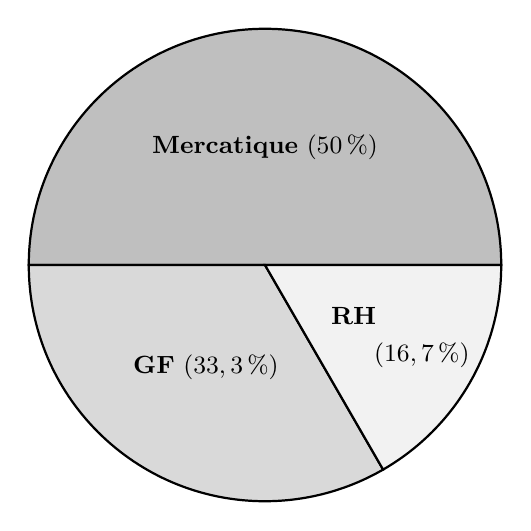
\begin{tikzpicture}[baseline=(current bounding box.center)]
			\fill[gray!50] (0,0) -- (0:3) arc (0:180:3) -- cycle;
			\draw[thick] (0,0) -- (0:3) arc (0:180:3) -- cycle;
			\node at (90:1.5) {\small \textbf{Mercatique} ($50\,\%$)};
			\fill[gray!30] (0,0) -- (180:3) arc (180:300:3) -- cycle;
			\draw[thick] (0,0) -- (180:3) arc (180:300:3) -- cycle;
			\node at (240:1.5) {\small \textbf{GF} ($33,3\,\%$)};
			\fill[gray!10] (0,0) -- (300:3) arc (300:360:3) -- cycle;
			\draw[thick] (0,0) -- (300:3) arc (300:360:3) -- cycle;
			\node at (330:1.3) {\small \textbf{RH}};
			\node at (330:2.3) {\small ($16,7\,\%$)};
		\end{tikzpicture}
	\end{center}
\end{ex}

\newpage

\subsection{Caractère continu : Histogramme et Polygon des E.C.C.}

\begin{defin}[Histogramme]
	Pour une série regroupée en classes, l'\textbf{histogramme} est constitué de rectangles adjacents dont l'\textbf{aire} est proportionnelle à l'effectif de la classe.
\end{defin}

\begin{remarque}
	Si toutes les classes ont la même amplitude, la \textbf{hauteur} de chaque rectangle est alors directement proportionnelle à l'effectif.
\end{remarque}

\begin{ex}[Histogramme à classes d'amplitudes égales]
	On reprend la taille des $24$ élèves de STMG regroupés par classes de $5\text{ cm}$ :
	\begin{center}
		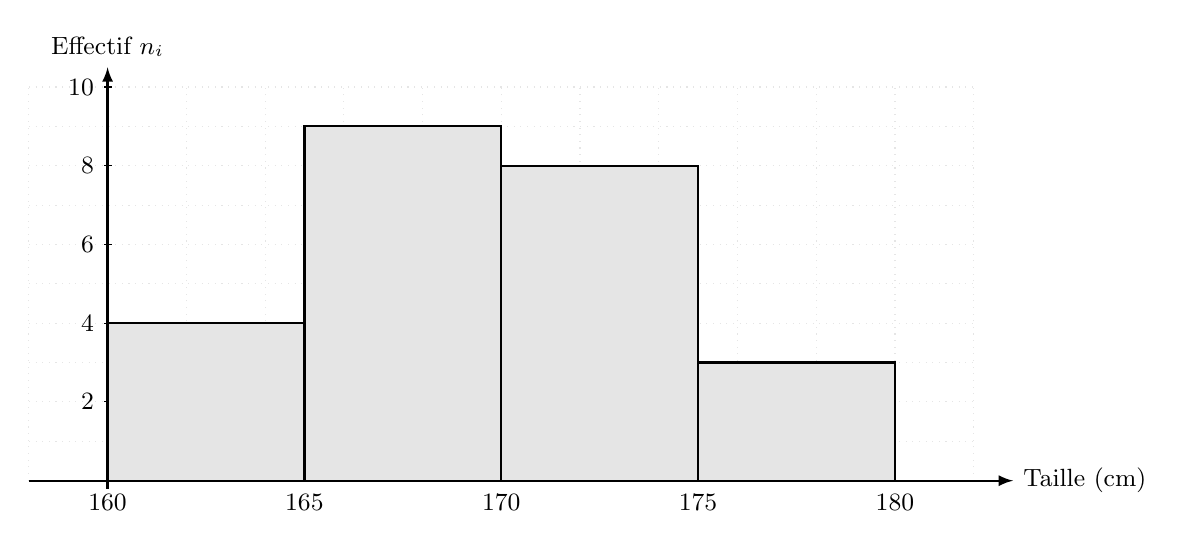
\begin{tikzpicture}[scale=0.5, baseline=(current bounding box.center)]
			\draw[gray!20, dotted] (158,0) grid[xstep=2, ystep=1] (182,10);
			\draw[->, >=latex, thick] (158,0) -- (183,0) node[right] {\small Taille (cm)};
			\draw[->, >=latex, thick] (160,-0.2) -- (160,10.5) node[above] {\small Effectif $n_i$};
			\foreach \y in {2,4,6,8,10} { \draw (160.1,\y) -- (159.9,\y) node[left] {\small \y}; }
			\draw[fill=gray!20, thick] (160,0) rectangle (165,4);
			\draw[fill=gray!20, thick] (165,0) rectangle (170,9);
			\draw[fill=gray!20, thick] (170,0) rectangle (175,8);
			\draw[fill=gray!20, thick] (175,0) rectangle (180,3);
			\foreach \x in {160,165,170,175,180} { \node[below] at (\x,-0.1) {\small \x}; }
		\end{tikzpicture}
	\end{center}
\end{ex}

\subsection{Polygone des effectifs cumulés croissants (E.C.C.)}

\begin{defin}[Polygone des E.C.C.]
	Le \textbf{polygone des effectifs cumulés croissants} (ou des fréquences cumulées croissantes) permet de visualiser la répartition cumulée des données d'un caractère continu.
	\begin{itemize}
		\item On place les points dont l'\textbf{abscisse} est la borne supérieure de la classe et l'\textbf{ordonnée} est l'E.C.C. (ou la F.C.C.) correspondant.
		\item On relie ces points par des segments de droite, en partant du point correspondant à la borne inférieure de la première classe d'ordonnée $0$.
	\end{itemize}
\end{defin}

\begin{ex}[Tracé du polygone des E.C.C. et détermination graphique de la médiane]
	On reprend le tableau des tailles des $24$ élèves de STMG :

	\begin{center}
		\rnc{\arraystretch}{1.3}
		\begin{tabular}{|>{\columncolor{gray!30}}c|c|c|c|c|} \hline
			Classes $[a ; b[$ & $[160 ; 165[$ & $[165 ; 170[$ & $[170 ; 175[$ & $[175 ; 180[$ \\ \hline
			Effectifs $n_i$   & 4             & 9             & 8             & 3             \\ \hline
			E.C.C.            & 4             & 13            & 21            & 24            \\ \hline
		\end{tabular}
	\end{center}

	Les points à placer sont : $(160 ; 0)$, $(165 ; 4)$, $(170 ; 13)$, $(175 ; 21)$ et $(180 ; 24)$.

	\begin{center}
		\begin{tikzpicture}[scale=0.4, baseline=(current bounding box.center)]
			\draw[gray!90, dotted] (158,0) grid[xstep=2, ystep=2] (182,26);
			\draw[->, >=latex, thick] (158,0) -- (183,0) node[right] {Taille (cm)};
			\draw[->, >=latex, thick] (158,-0.2) -- (158,26.5) node[above] {E.C.C.};
			\foreach \y in {0,4,8,12,16,20,24} { \draw (158.3,\y) -- (157.7,\y) node[left] {\y}; }
			\draw[line width=0.5mm, gray, mark=*] plot coordinates { (160,0) (165,4) (170,13) (175,21) (180,24) };
			\draw[dashed, thick, ->] (158,12) -- (169.44,12);
			\draw[dashed, thick, ->] (169.44,12) -- (169.44,0);
			\node[left, xshift=-12mm] at (160,12) {$\dfrac{N}{2}\rarr$};
			\node[below, yshift=-6mm] at (169.44,0) {$M_e \approx 169,4$};
			\foreach \x in {160,165,170,175,180} { \draw (\x,-0.2) -- (\x,0.2); \node[below] at (\x,-0.1) {\x}; }
		\end{tikzpicture}
	\end{center}

	\begin{rem}
		Sur le polygone des E.C.C., l'abscisse correspondant à l'ordonnée $\dfrac{N}{2} = 12$ donne une estimation graphique de la \textbf{médiane} $M_e \approx 169{,}4\text{ cm}$.
	\end{rem}
\end{ex}
